\documentclass[9pt,twocolumn,twoside]{pnas-new}
% Use the lineno option to display guide line numbers if required.
% Note that the use of elements such as single-column equations
% may affect the guide line number alignment.
\templatetype{pnasresearcharticle} % Choose template
% {pnasresearcharticle} = Template for a two-column research article
% {pnasmathematics} = Template for a one-column mathematics article
% {pnasinvited} = Template for a PNAS invited submission
%\usepackage{graphicx}

\usepackage{amsmath,amsfonts,amssymb}
\usepackage{fullpage}
\usepackage{color}
\usepackage{bm}
\newcommand{\rr}[1]{{\rm #1}}



% \usepackage[english]{babel}
% \usepackage[latin1]{inputenc}
% \usepackage[T1]{fontenc}
% \usepackage{color}
% \usepackage{float}
% \usepackage{verbatim}
% \usepackage{graphicx}
% \usepackage{bm}
% \usepackage{mathtools}
% \usepackage{stmaryrd}
% \usepackage{anyfontsize}
% \usepackage{fullpage}
% \usepackage{color}


% \graphicspath{{../Enigma/figures/}}



% \title{Quantization of ecological interactions yields insights into ecosystem assembly and dynamics}
\title{Diverse interactions and ecosystem engineering stabilize assembly of ecological networks}

% Use letters for affiliations, numbers to show equal authorship (if applicable) and to indicate the corresponding author
\author[a,b]{Justin D. Yeakel}
% \author[a,b]{Hattie}
\author[c]{Mathias Pires}
\author[c]{Marcus A. M. de Aguiar}
\author[d]{James O'Donnell}
\author[e]{Paulo R. Guimar\~aes Jr.}
\author[f]{Dominique Gravel}
\author[g]{Thilo Gross}


\affil[a]{School of Natural Sciences, University of California Merced, Merced, CA 95343, USA}
\affil[b]{Santa Fe Institute}
\affil[c]{Universidade Estadual de Campinas}
\affil[d]{University of Washington}
\affil[e]{Universidade de S\~ao Paulo}
\affil[f]{Universit\`e de Sherbrooke}
\affil[g]{University of California Davis, Davis CA}

% Please give the surname of the lead author for the running footer
\leadauthor{Yeakel}

% Please add here a significance statement to explain the relevance of your work
\significancestatement{
Here
%Authors must submit a 120-word maximum statement about the significance of their research paper written at a level understandable to an undergraduate educated scientist outside their field of speciality. The primary goal of the Significance Statement is to explain the relevance of the work in broad context to a broad readership. The Significance Statement appears in the paper itself and is required for all research papers.
}

% Please include corresponding author, author contribution and author declaration information
\authorcontributions{Please provide details of author contributions here.}
\authordeclaration{Please declare any conflict of interest here.}
\correspondingauthor{\textsuperscript{2}To whom correspondence should be addressed. E-mail: jyeakel@ucmerced.edu}

% Keywords are not mandatory, but authors are strongly encouraged to provide them. If provided, please include two to five keywords, separated by the pipe symbol, e.g:
\keywords{Ecosystem assembly $|$ Ecological networks $|$ Colonization $|$ Extinction $|$ Ecosystem engineering}
\begin{abstract}
Some cool shit.
\end{abstract}
\dates{This manuscript was compiled on \today}
\doi{\url{www.pnas.org/cgi/doi/10.1073/pnas.XXXXXXXXXX}}



\begin{document}
% Optional adjustment to line up main text (after abstract) of first page with line numbers, when using both lineno and twocolumn options.
% You should only change this length when you've finalised the article contents.
\verticaladjustment{-2pt}

\maketitle
\thispagestyle{firststyle}
\ifthenelse{\boolean{shortarticle}}{\ifthenelse{\boolean{singlecolumn}}{\abscontentformatted}{\abscontent}}{}


%structure is the result of dynamics
To unravel nature's secrets we must simplify its abundant complexities and eccentricities.
% Simplifying the abundant complexities and eccentricities of nature is necessary to unravel its secrets.
The layers of natural history giving rise to an ecological community can be distilled -- among many forms -- into a network, where nodes represent species and links represent interactions between them.
In the past the necessary simplifications meant that networks were typically constructed for one type of interaction, such as food webs, capturing predation \cite{Paine1966,Dunne2002,Pascual2006}, or pollination networks capturing a specific mutualistic interaction \cite{Bascompte2013}. 
While this has led to significant breakthroughs \cite{May1972,Gross2009,Allesina2012}, recent interest in `multilayer networks', comprising multiple interaction types has been gaining momentum \cite{Kefi2016,Pilosof2017}. 
However, still difficult to accommodate are interactions where species affect others by altering the environment in a lasting way. 
These interactions, labeled ecosystem engineering \cite{Lawton1994,OdlingSmee2013}, are quite common in nature and exist in almost every ecosystem.

% This minimalist perspective provides insight into community structure \cite{Dunne2002,Pascual2006}, and consequently, the dynamics of populations and system stability \cite{May1972,Gross2009,Allesina2012}.
% Community structure can directly impact the ability of the system to absorb external perturbations \cite{Novak2011,Aufderheide2013,Novak2016}, the existence and ubiquity of tipping points marking sudden changes in species' populations \cite{Lade2011,Boettiger2012}, and promote or inhibit extinction cascades \cite{Stouffer2011,Yeakel2014}.
% Importantly, community structure is the result of a dynamical process that takes place over time, where species are added to or removed from the community in succession \cite{Weiher2001}.
% This process is generally referred to as community assembly, and though it is an engine for much that we observe in nature, is not well understood.

%multiple interaction types
% Ecological networks are generally constructed and analyzed with respect to a single type of interaction.
% For example, beneficial relationships between species form the foundation of mutualistic networks, whereas antagonistic interactions form the foundation of trophic networks, or food webs. %- which are often trophic in one direction and a reproductive service in the other -
% There has been a growing interest in understanding community structure by taking into account diverse interaction types \cite{Kefi2016}, where multiple unique interactions are included, sometimes in a multi-layer network \cite{Pilosof2017}.
% Interactions between two species are inherently compound in nature, such that both species in an interaction experiences different effects.
% For example, mutualistic interactions generally involve a flow of biomass in one direction and a reproductive service in the other; in a trophic interaction there is a flow of biomass from the prey to the predator but not the reverse.
% This asymmetry is generally encoded into the dynamics, rather than the network structure itself \cite{Gross2009,Allesina2012}.


%Ecosystem engineering
Diverse interactions occur not only between species, but indirectly through the effects that species have on their environment \cite{Jones1994,Olff2009,OdlingSmee2013}.
An organism that alters the environment on timescales longer than its lifetime is known as an ecosystem engineer \cite{Hastings2007}.
In contemporary systems, ecosystem engineers are relatively common and can alter the landscape on which ecological interactions occur \cite{Wright2006}.
Thereby elephants root out large saplings and small trees, enabling the formation and maintenance of grasslands \cite{Haynes2012} and creating habitat for smaller vertebrates \cite{Pringle2008}.
Burrowing rodents create shelter and promote primary production by aerating the soil \cite{Reichman2002}, salmon and aquatic invertebrates create freshwater habitats by changing stream morphology \cite{Moore2006}, and leaf-cutter ants alter microclimates, influencing seedling survival and plant growth \cite{Meyer2011}.

Ecosystem engineering not only impacts communities on ecological timescales, but has profoundly shaped the evolution of life on Earth.
For example, the emergence of multicellular cyanobacteria fundamentally altered the atmosphere during the Great Oxidation Event of the Proterozoic roughly 2.5 Byrs BP \cite{Schirrmeister2013}, paving the way for the invasion of terrestrial habitats.
In the oceans, it is thought that rRNA and protein biogenesis of aquatic photoautotrophs drove the nitrogen:phosphorous ratio (the Redfield Ratio) to ca. 16:1, matching that of plankton \cite{Loladze2011}.
% While local habitats can be significantly impacted by single engineering species, larger scale effects are generally modified by diverse engineering clades.
While engineering species such as elephants can have considerable impact on local environments, engineering clades can have much larger, sometimes global-scale, effects.


% These example describe indirect interactions between ecosystem engineers and species that rely on their engineering, through an environmental intermediary.
% By way of their indirectness, these interactions are difficult to document.

% GLOBAL SHIFTS ORIGINATE DUE TO ENGINEERING BY A LARGE GROUP OF RELATED SPECIES


% 
% Recent efforts have examined engineering through the lens of niche construction \cite{Krakauer2009}, such as the construction of shared resources such as metabolite in microbiotic communities \cite{Kallus2017}.
% Engineering by way of niche construction is a strategy that may be evolutionary precarious \cite{Krakauer2009}, but may also serve as the missing ingredient that stabilizing some complex ecological systems \cite{Muscarella2017}.

%NOTE: From THILO
% The effect of the abiotic environemt on the lifeforms is commonly included in models because it is felt to be important and can (at least to first approximation) be easily systematized. By compaison the way in which species engineer the environment defies easy systemization due to the multitude of mechanisms by which the engineering occurs. Despite being perhaps of equal importnace engineering is hence omitted from most models. 



The effect of the abiotic environment on species is commonly included in models of ecological dynamics \cite{Woodward2010,Brose2012,Gibert2019b} both due to its acknowledged importance and because it can -- to first approximation -- be easily systematized. 
By comparison the way in which species engineer the environment defies easy systemization due to the multitude of mechanisms by which engineering occurs.
% Despite its relevance, the interactions facilitated by ecosystem engineers have not been included in models of ecological networks.
% Interactions between species and the abiotic environment have been conceptually described \cite{Olff2009,Getz2011}, however how these effects impact community function has not been explored.
While interactions between species and the abiotic environment have been conceptually described \cite{Olff2009,Getz2011}, the absence of engineered effects in ecological networks was addressed by Odling-Smee et al. \cite{OdlingSmee2013}, where they outlined a conceptual framework that included both species and abiotic compartments as nodes of a network, with links denoting both biotic and abiotic interactions.
% Importantly, they emphasize the potential eco-evolutionary consequences of prior alterations to the environment influencing an ecological system at some future state.


%HERE WE...
Here we model an ecological system as a network where nodes represent ecological entities, including engineering species, non-engineering species, and the effects of the former on the environment, which we call \emph{objects}.
The links of the network that connect both species and objects represent trophic (eat interactions), service (need interactions), and engineering dependencies, respectively (Fig. \ref{fig:model}; see Materials and Methods for a full description).
Objects in our framework overlap conceptually with the `abiotic compartments' described in Odling-Smee et al. \cite{OdlingSmee2013}.
Following Pillai et al. \cite{Pillai2011}, we do not track the abundances of entities but only track their presence or absence.
We use this framework to explore the dynamics of ecosystem assembly, where the colonization and extinction of species within a community depends on the constraints imposed by the trophic, service, and engineering dependencies.
Because ecological assembly is not a memory-less process, it is likely that engineers can have considerable impact on the emergence of community structure and dynamics.

Our results offer four key insights into the roles of diverse interactions and ecosystem engineering in driving community assembly.
First, we show that the assembly of species networks in the absence of engineering reproduces many features observed in empirical systems.
These include changes in the proportion of generalists over the course of assembly that accord with measured values, and trophic diversity similar to empirical observations. % both maximum trophic level and 
Second, we show that increasing the frequency of mutualistic interactions leads to the assembly of ecological networks that are more nested, a hallmark feature of mutualistic systems \cite{Bascompte2003}.
However, we also observe that increased mutualistic dependencies in the assembled communities lower species' persistence.
This suggests that while nested mutualistic networks appear to be dynamically favored (cf. Ref. \citenum{Rohr2014}), our model predicts that the additional inter-dependencies associated mutualisms should will lead to greater species turnover and changes in community composition.

%3: Engineering - moderate amounts increase extinction rates, but large amounts decrease extinction rates. The role of dependencies and redundancies
We next explore the effects of ecosystem engineering on the dynamics of community assembly.
Our third key result shows that increasing both the number of ecosystem engineers and engineering interactions within a community has nonlinear effects on observed extinction rates.
While we find that a low amount of engineering increases extinction rates, a high amount of engineering serves to reduce extinction rates due to the large niche space facilitated by engineers.
Finally, we show that the inclusion of engineering modifies the effects of mutualistic interactions, and can reduce the negative effects that mutualisms have on species' persistence.\\
% Only by understanding the effects of engineers on communities can we gain insight into 

% 
% %Model description: Pool, colonization, extinction (interaction strength), objects
% \noindent \textbf{Assembly of the ENIgMa network}\\
% A combination of two directional interactions between a pair of species defines the ecological relationship linking both.
% % As such, the trophic and mutualistic interactions mentioned above can be deconstructed into two directional interactions.
% A mutualistic interaction between plant x and pollinator y can thus be deconstructed into an `eat' interaction from species x to y and a \emph{need} interaction from species y to x.
% The former represents a directional trophic interaction, or a resource dependency, whereas the latter represents a reproductive service, or a dependency that does not involve biomass flow.
% Another type of mutualism is one defined by non-resource dependencies for both species, often called a service-service mutualism.
% In this case, each species would be connected to the other by directional \emph{need} interactions.
% A trophic interaction between species x and y can be deconstructed by an \emph{eat} interaction from the consumer x to the prey y, but the absence of an interaction from prey y to the consumer x, as the prey does not interact meaningfully with the consumer.
% Some species pairs may participate in bi-directional trophic interactions, where the consumer/resource role changes over the course of each species' life history.
% In this case, each species would be connected to the other by directional \emph{eat} interactions.
% 
% 
% %Interactions with both species and the environment (engineering)
% Ecosystem engineering can be formalized by the creation of an object by an engineering species that can be interacted with by other members of a community.
% Objects made by ecosystem engineers represent any alteration made to the environment, whether this be changes to the stoichiometry of the atmosphere (e.g. primary producers; refs), physical modifications to the landscape (e.g. beavers, salmon; refs), or the production of unique habitats for other organisms (e.g. tree trunks; refs).
% Objects can be represented in ecological network alongside species as nodes, but where they must be connected to engineering species by a \emph{make} interaction.
% The \emph{make} interaction between an engineering species and the engineered object denotes the dependency of the environmental effect on the effector.
% 


%Food webs
\noindent \textbf{Trophic assembly without engineering} \\
\noindent Communities assemble by colonization from a source pool, and extinction due to competitive exclusion. 
Colonization is possible if a species can fulfill $\geq 1$ trophic requirement and all of its service requirements.
Following the establishment of an autotrophic base, mixotrophs and lower trophic heterotrophs comprise the initial colonizers, succeeded by higher trophic consumers.
Primary extinctions occur by the competitive exclusion of species sharing similar resources.
A species' competition strength is determined by its interactions: competition strength is enhanced by the number of its mutualistic partners and penalized by its trophic generality (number of prey) and vulnerability (number of predators).
Secondary extinctions occur when species lose their trophic or service requirements.
As the colonization and extinction rates converge, the community reaches a steady state around which it oscillates stochastically.
see Materials and Methods for a complete description of the assembly process. % due to losses from primary extinctions.
% As species richness increases, competitive exclusion initiates the extinction process, followed by secondary extinctions due to the loss of trophic and service requirements among species.


\begin{figure}
\centering
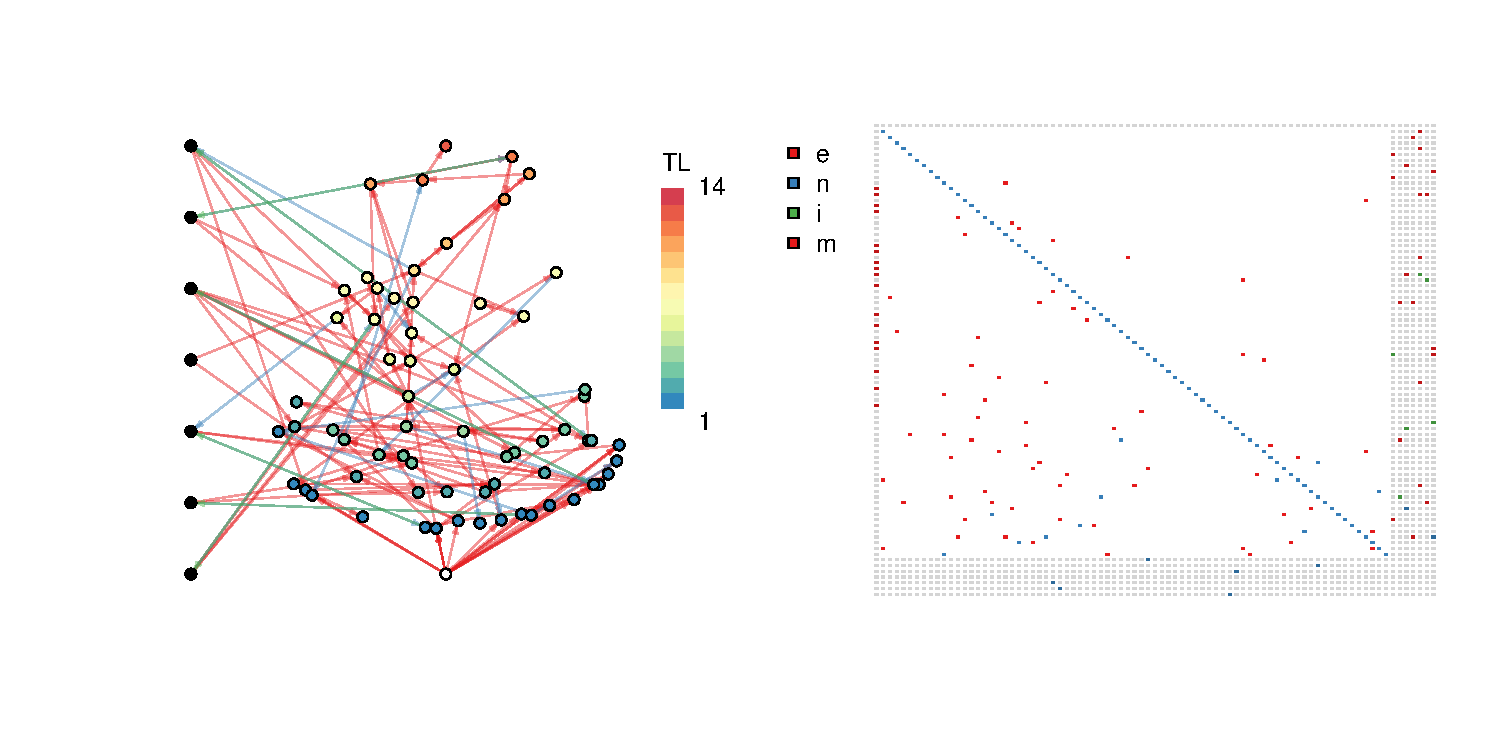
\includegraphics[width=0.5\textwidth]{fig_model.pdf}
\caption{
A. Diverse interactions between species (colored nodes) and abiotic objects (black nodes)
B. An assembling food web with species (colored nodes) and objects (black nodes). The basal resource is the white node rooted at the bottom of the network.
C. The corresponding adjacency matrix with colors denoting interactions between biotic (species) and abiotic (objects) entities. The basal resource is denoted in row/column 1. 
}
\label{fig:model}
\end{figure}


% 1) connectance
Assembly of ecological communities in the absence of engineering results in interaction networks with structures consistent with observations of empirical systems.
As the community reaches steady state, we find that the connectance of trophic interactions ($C=L/S^2$, where $S$ is species richness and $L$ is the number of links in the community) begins high and then decays to a value similar to that of the source pool.
% The species richness of the community increases to $S_{\bm A}=130$.
Decaying connectance has been documented in the assembly of mangrove communities \cite{Piechnik2008}, however this decay is a statistical inevitability, as a growing food web early in the assembly process must have high link density (few species that are fully connected) from which it can only decline.
% That the connectance of assembled communities is greater than the source pool is due to the fact that only species connected by trophic interactions can enter the community to begin with, increasing expected link density compared to the overall pool.
Compared to trophic networks constructed using the Niche model \cite{Williams2000} given equal species richness and connectance, our framework results in networks with degree distributions of similar means but with reduced variance (Supplementary Information: Appendix I).

% 
% \begin{figure}
% \centering
% 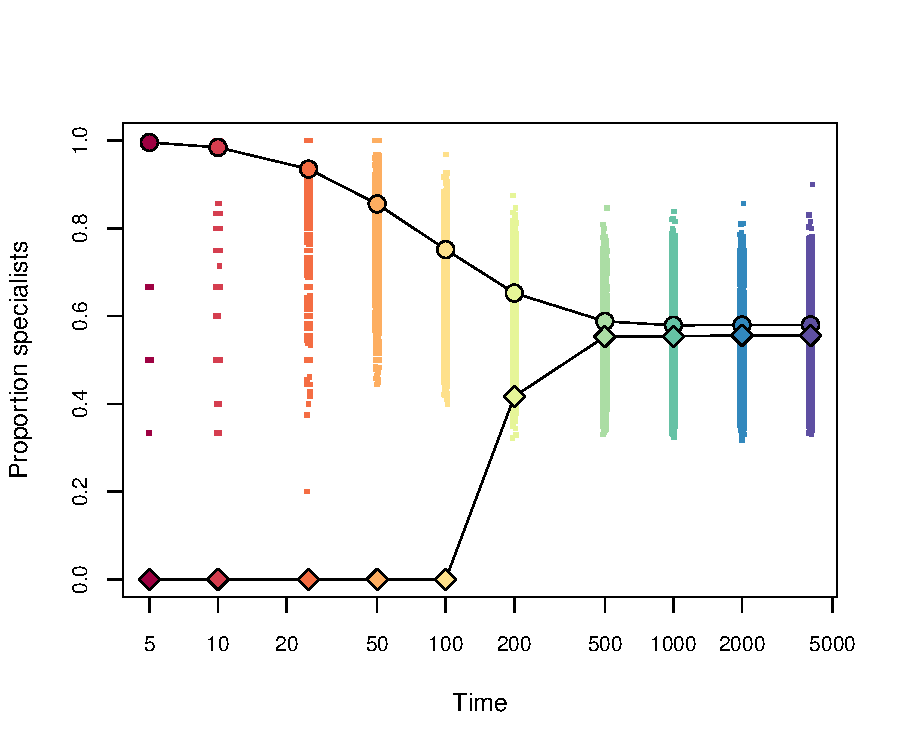
\includegraphics[width=0.5\textwidth]{fig_specialization.pdf}
% \caption{
% The proportion of specialists as a function of assembly time, where a specialist is defined as a species with a generality index $G_i < 1$.
% All measures of $G_i$ are scaled by the average number of links per species $L/S$, and we consider different values of $L/S$ on $G_i$:
% Circles: $G_i^{\rr{all}}$ where $L$ accounts for all links in the food web and $S$ accounts for all species relative to each time interval in the assembly process (averaged across replicates);
% Points: $G_i^{\rr{hetero}}$, where we consider only the links and species richness of heterotrophs, excluding autotrophs (each point shows an individual replicate);
% Diamonds: $G_i^*$, where $L$ and $S$ are measured with respect to the communities at steady state, which is most similar to the measure used to evaluate assembling mangrove food webs (averaged across replicates).
% }
% \label{fig:spec}
% \end{figure}




%Generality
Recent empirical work has suggested that generalist species may play an important role early in community assembly, whereas specialists tend to colonize after a diverse resource base has accumulated \cite{Piechnik2008}.
Here, the trophic generality for a species $i$ is defined as $G_i = \sum_{j}A_{i,j}(L/S)^{-1}$, where $A$ is the adjacency matrix of trophic interactions such that the summation is the number of resources consumed by species $i$ \cite{Williams2000}.
A species is classified as a generalist if the number of its trophic interactions is greater than the average number of links per species, $L/S$, such that $G_i > 1$ and a specialist if $G_i < 1$.
% The trophic breadth of potential colonizers is thought to play an important role in community assembly.
% Because the definition of a specialist or generalist to some degree depends on the size and connectance of the larger food web, trophic generality can be defined as $G_i = \sum_j \rr{e}_{{\bm A}(i,j)}(L/S)^{-1}$, such that the number of trophic interactions for a consumer is scaled by the average number of trophic interactions per species in the community $L/S$ (Piechnik, others).
% A species is classified as a generalist if the number of its trophic interactions is greater than the average number of links per species, or $G_i > 1$, and a specialist if $G_i < 1$, where a community can be described by the proportion of specialists found therein. %$\rho_\rr{s}(G)$
% For interaction networks that are assembling over time, generality can be scaled by a number of different measures of $L/S$, and this has a large effect on our interpretation of the role of generality in community assembly.
% For instance, $L/S$ may be quantified by either including all autotrophic species or only autotrophic functional groups.
% Furthermore, the scaling of generality may be made with respect to the current state of the community at each point in time, or with respect to the community at steady state.
% For instance, in their investigation of assembling mangrove food webs (originally described by Simberloff, xxx), Piechnik et al. (2008) scaled trophic breadth to a standard steady state value of $L^*/S^* = 0.2$ averaged across 102 food webs.
% To examine how our assessment of the role of generalism over the course of assembly changes based on the application of different scalings, we employ three different measures of $L/S$ to calculate $G_i$:
% 1) $G_i^{\rr{all}}$, where $L$ accounts for all links in the food web and $S$ accounts for all species relative to each time interval in the assembly process (circles; Fig. \ref{fig:spec}b);
% 2) $G_i^{\rr{hetero}}$, where we consider only the links and species richness of heterotrophs, excluding autotrophs (points; Fig. \ref{fig:spec}b);
% 3) $G_i^*$, where $L$ and $S$ are measured with respect to the communities at steady state, which is most similar to the measure used to evaluate assembling mangrove food webs (diamonds; Fig. \ref{fig:spec}b).
% Whether trophic breadth is scaled to the current state of $L/S$ or the steady state value of $L^*/S^*$ has a large influence on the estimated proportion of generalists in the community, particularly when the size of the system is small.
% We observe that for $G_i^{\rr{all}}$, the system is initially assembled by specialist species, though over the course of assembly the proportion of specialists relative to generalists declines to intermediate values (circles representing the average over replicates in Fig. \ref{fig:spec}).
% If only the trophic links between non-autotrophs are considered as in $G_i^{\rr{hetero}}$, specialists still dominate early in assembly, but there is a greater range, such that some systems can be described by a mixed proportion of specialists and generalists (individual points representing independent replicates in Fig. \ref{fig:spec}).
Following Piechnick et al. \cite{Piechnik2008}, if generalism is scaled to the steady state link density, we observe that generalists dominate early in assembly, with an increase in specialists as assembly progresses (Fig. \ref{fig:trophic}A).
At steady state the proportion of specialists levels out at ca. 60\%, similar to empirical observations of assembling mangrove communities.
%, all measures of $L/S$ are approximately equivalent, and


%trophic levels
%Trophic Levels & degree dists
The role of specialists early in assembly is primarily due to the accumulation of autotrophs specializing on the basal resource.
This is evident when we observe that the trophic level (TL) distribution early in assembly ($t=5$) has an average ${\rm TL}=1.6$.
% Additional consumers arrive in the form of both mixotrophs (consuming the basal resource and one or more autotrophs) and heterotrophs, which establish higher trophic levels.
Four trophic levels are typically established by $t=50$, where colonization is still the dominant dynamic, and by the time communities reach steady state the interaction networks are characterized by an average ${\rm TL_{max}}$ ($\pm$ standard deviation) $=11 \pm 2.8$ (Fig. \ref{fig:trophic}B).
While the maximum trophic level is higher than that measured in most predator-prey systems (ref), it is not unreasonable if parasitic interactions (which we do not differentiate from other consumers in our framework) are included \cite{Lafferty2006}.
Overall, the most common trophic level among species at steady state is ca. ${\rm TL}=4.75$.

The distribution of trophic levels changes shape over the course of assembly.
early in assembly, we observe that the community exhibits a skewed pyramidal structure, where most species richness feeds from the base of the food web.
At steady state, we observe that intermediate trophic levels dominate, with frequencies taking on an hour-glass structure.
Compellingly, the trophic richness pyramids that we observe at steady state follow closely the hourglass distribution observed for empirical food webs and are less top-heavy than those produced by static food web models \cite{Turney2016}.\\




% We emphasize that these structures are diversity-weighted rather than biomass or abundance-weighted as is often the case \cite{Trebilco2013,Gibert2019}.
% Trophic levels higher than 7 do occur, but are rare.

%Cascading extinctions: Thebault
%Assembly patterns: Barbier
%Origin of ecological structure: Stokstad


%Drossel
% [RELATE TO TROPHIC ASSEMBLY MODELS]\\
%Hourglass food webs are predicted for systems where body size increases with trophic position (marine systems)



% 4) Increased mutualisms => greater nestedness
\noindent \textbf{Structure and dynamics of mutualisms} \\
Nested interactions, where specialist interactions are subsets of generalist interactions, are a distinguishing feature of mutualistic networks \cite{Bascompte2003}.
Moreover, nested interactions have been shown to maximize the structural stability of mutualistic networks \cite{Rohr2014}, emerge naturally via adaptive foraging behaviors \cite{Valdovinos2016,Valdovinos2019}, and promote the influence of indirect effects in driving coevolutionary dynamics \cite{Guimaraes2017}.
While models and experiments of trophic networks suggest that compartmentalization confers greater stabilizing properties \cite{Stouffer2011,Gilarranz2017}, interaction asymmetry among individuals may promote nestedness in both trophic \cite{Araujo2010} and mutualistic systems \cite{Pires2011}.
Processes that operate on different temporal and spatial scales may have a significant influence on these observations \cite{Massol2011}.
For example, over evolutionary time, coevolution and speciation may degrade nested structures in favor of modularity \cite{Ponisio2019}, and there is some evidence from Pleistocene food webs that geographical insularity may reinforce this process \cite{Yeakel2013}.

\begin{figure}[h!]
\centering
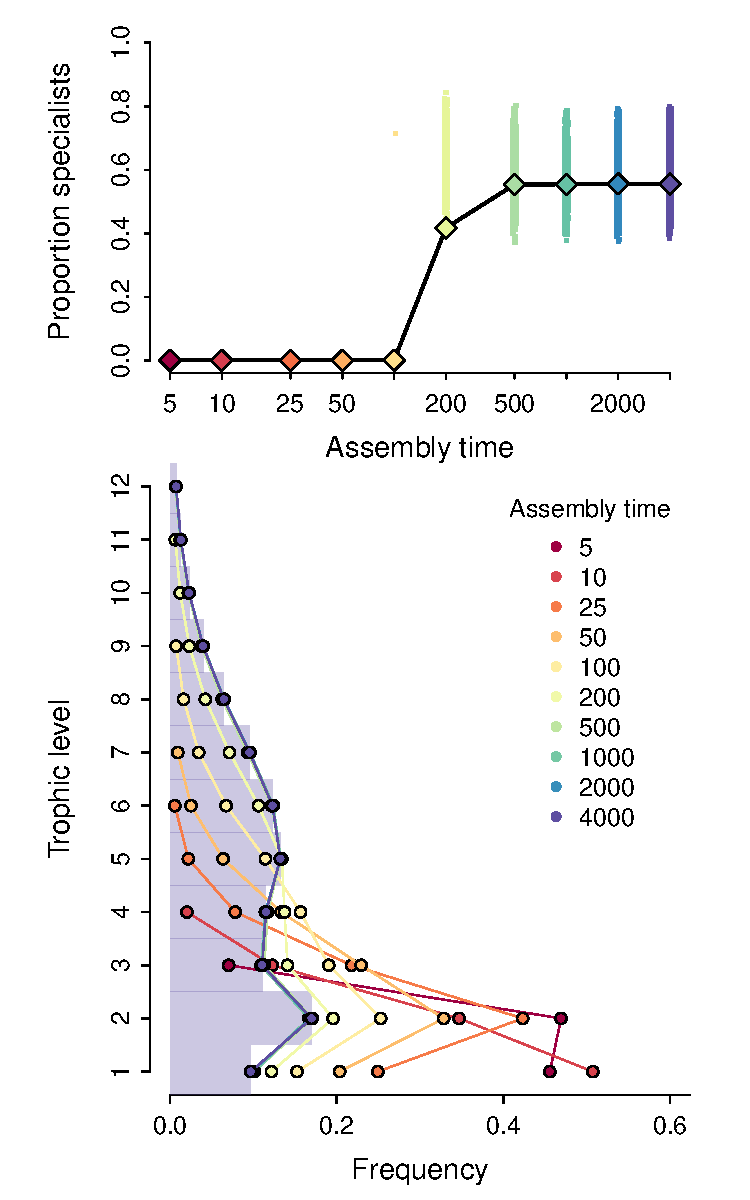
\includegraphics[width=0.4\textwidth]{fig_trophic.pdf}
\caption{
A. The proportion of specialists as a function of assembly time, where a specialist is defined as a species with a generality index $G_i < 1$.
All measures of $G_i$ are scaled by the average number of links per species where $L$ and $S$ are measured with respect to the communities at steady state.
B. The frequency distribution of trophic levels over the course of assembly taken across $10^4$ replicates. Autotrophs occupy trophic level 1.
We set $S=200$, $p_e=0.01$, $p_n=0.002$, and $t=4000$ (see Materials and Methods).
}
\label{fig:trophic}
\end{figure}


Does the assembly of ecological networks favor nested structures in systems where there are more mutualistic interactions between species?
Increasing service dependencies (need interactions; see Fig. \ref{fig:model}) leads to a higher frequency of both service-resource and service-service dependencies.
These interactions alter two key dynamics in our model: more service interactions \emph{i}) increases a species' competition strength, which will lower its probability of primary extinction, while also \emph{ii}) increasing inter-species dependencies, potentially increasing the likelihood of secondary extinctions.
% As such, elimination of a species that provides a service will result in the secondary extinction of the species that receives that service.
While mutualisms must carry with them fitness advantages in order to evolve, the latter dynamic highlights the potential risk associated with losing mutualistic partners \cite{Bond1994,Colwell2012}.
Indeed, the precarious balance that mutualists must maintain by way of their dependencies may have large implications for the future of global biodiversity \cite{Dunn2009}.

We find that as we increase the frequency of mutualistic interactions, the assembled community at steady state becomes more nested (Fig. \ref{fig:nest}).
% That the absolute values of nestedness are low compared to those measured for empirical mutualistic networks is unsurprising: observations of mutualistic interactions are generally for bipartite networks and isolated to specific systems (e.g. ant-plant mutualisms).
% Here the NODF metric is taken across both eat and need interactions across the entire assembled community.
In this case, nestedness is both the outcome of the assembly process as well as a stabilizing structure.
We observe this by examining the differences in competition strength between species in mutualistic versus trophic networks in a simple nested motif (Fig. \ref{fig:nest}, inset).
In trophic networks, species with many predators (high vulnerability) are at greater risk of competitive exclusion.
Their elimination will have a larger effect on multiple consumers internal to the nested structure, rendering it prone to disturbance.
In mutualistic networks, species with many predators gain the competitive advantages of services.
If the benefit of mutualisms to competition strength is greater than the cost of vulnerability (as described in Materials and Methods), it is the low vulnerability species consumed by fewer predators that are at greater risk of competitive exclusion.
Their elimination will affect fewer consumers external to the nested structure, rendering it more resistant to disturbance.


Our results also suggest that the addition of mutualistic interactions comes at a cost.
Because mutualisms increase dependencies between species, and by extension the frequency of secondary extinctions, we observe that these networks have lower species' persistence (Fig. \ref{fig:nest}). %as well as lower diversity (Supplemental Materials).
% both lower species diversity on average as well as lower species' persistence.
Persistence is defined by the percent simulation time a given species is present in the community, such that lower persistence means greater species turnover.
In fact, assembling plant-pollinator systems have demonstrated high rates of species and interaction turnover, seemingly independent of whether the system was actively assembling or had reached a steady state \cite{Ponisio2017}.
An important limitation of our framework is that we do not allow for flexible mutualistic interactions; a species must satisfy all of its service requirements to remain in the community.
Relaxing these assumptions permits mutualism plasticity, long considered to be an important component driving the structure of mutualistic interactions \cite{Ramos2012,Valdovinos2016,Ponisio2017,Valdovinos2019}, which may be a fruitful perspective for future investigation.\\
%What is the CV of mutualistic trajectories?



\begin{figure}
\centering
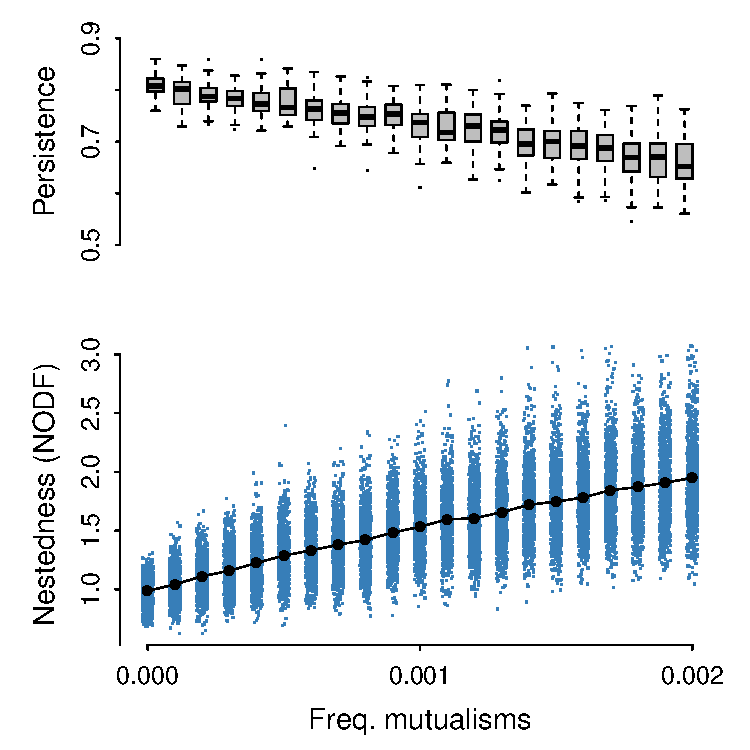
\includegraphics[width=0.5\textwidth]{fig_nested.pdf}
\caption{
A. Species persistence and
B. Nestedness (measured as NODF) for communities with increasing frequencies of mutualistic (service) interactions.
}
\label{fig:nest}
\end{figure}

\noindent \textbf{Community assembly with ecosystem engineers} \\
%Theory
Models that explore the effects of ecosystem engineering are relatively few, but have covered important ground \cite{Hastings2007,OdlingSmee2013}.
Initial work focused on understanding how habitat modification might impact the persistence of engineering species \cite{Gurney1996}, while more recent efforts have shown that engineering can promote invasion \cite{Cuddington2004} and impact primary productivity \cite{Wright2004}.
On eco-evolutionary timescales, ecosystem engineering can alter the selective environment \cite{Krakauer2009,OdlingSmee2013} and ultimately lead to unexpected outcomes such as the fixation of deleterious alleles \cite{Laland1999}.
% On macroevolutionary timescales, there is considerable interest in understanding the role of innovation on diversification and extinction rates within and among clades \cite{Marshall2016}.
% While such innovation generally pertains to the appearance of morphological traits, environmental modifications that result from evolutionary innovations can sometimes be wide-ranging, such as the planetary-scale consequences following the evolution of multicellular cyanobacteria \cite{Schirrmeister2013}.
On smaller scales, microbiota construct shared metabolitic resources that have a significant influence on microbial communities \cite{Kallus2017}, the dynamics of which may even serve as the missing ingredient stabilizing some complex ecological systems \cite{Muscarella2017}.


We next explore the effects of ecosystem engineering by allowing species to produce abiotic objects as additional nodes in the ecological network (Fig. \ref{fig:model}).
These object nodes produced by engineers can serve to fulfill resource or service requirements for other species.
The parameter $\eta$ defines the mean number of objects produced by each species, drawn from a Poisson distribution (see Materials and Methods for details).
Increasing the frequency of engineering interactions both increases the number of engineering species (those species that make $\geq 1$ object) and the number of objects made per species.
There are two characteristics of engineering that have particular relevance for community assembly:
objects can linger in the community even after the species that produce them have been excluded, and
more than one engineer can produce the same object such that engineering redundancies increase with $\eta$.




%Engineering can produce positive feedback dynamics on engineers
%Positive feedback over evolutionary time => speciation/radiation
%Lead to engineering redundancies
%This may be rare as Lawton suggests, but appears to be quite common in the microbial world.
%In microbiomes, horizontal gene transfer can produce redundant engineering without radiations

%Lawton 1994: there may be sometimes redundancy in ecosystem engineers... (uses beaver to suggest that there is not)

%negative (introduces dependencies) then positive (introduces redundancies)
Increasing engineering has significant consequences on community stability, but these effects also are sensitive to the frequency of service interactions within the community.
We measure community stability from 
\emph{i}) rates of primary versus secondary extinctions,
\emph{ii}) species persistence, and 
\emph{iii}) steady state community diversity.
Primary extinctions result from the competitive exclusion of species, whereas secondary extinctions are those that occur as a direct result of the former.
All measures were averaged over each species within the community across assembly time.

% Increasing engineering has different effects on primary versus secondary extinctions.
As the number of engineers increase, mean rates of primary extinction are first elevated and then decline (Fig. \ref{fig:engineers}A).
This nonlinear effect of engineering on rates of primary extinction results from two competing forces.
Increased production of abiotic objects supplies consumers with additional resources, limiting secondary extinctions and promoting persistence (Fig. \ref{fig:engineers}B).
However, the stabilization of consumers ultimately results in increased vulnerability of prey species.
 % while also increasing the vulnerability of prey.
The cumulative effect is increased competitive exclusion of prey and higher rates of primary extinction, particularly when engineers are rare (Fig. \ref{fig:engineers}A).
The presence of abiotic objects limits the magnitude of extinction cascades.
% In contrast, rates of secondary extinction decline and species' persistence increase as engineering creates abundant niche space (Fig. \ref{fig:engineers}B).
% Lower species' persistence => species' turnover.
Higher rates of primary extinction coupled with lower rates of secondary extinction mean that extinctions are common, but do not result in large cascades, such that disturbances are compartmentalized.
As engineering becomes more common (higher $\eta$) available niche space expands, diluting competition and leading to lower rates of primary extinction.
Together, these results suggest that ecological networks are least stable when engineers are rare, and most stable when engineers are common.

%Mutualisms
Increasing the frequency of service interactions promotes both mutualisms as well as service interactions between species and engineered objects (Fig. \ref{fig:model}).
A topical example of the latter is the habitat provided to invertebrates by the recently discovered rock-boring teredinid shipworm (\emph{Lithoredo abatanica}) \cite{Shipway2019}.
Here, freshwater invertebrates are serviced by the habitat modifications engineered by the shipworm, linking species indirectly via an abiotic effect (object).
As the frequency of service interactions increases, the negative effects associated with few engineers is diminished (Fig. \ref{fig:engineers}A).
Increasing service interactions both elevates the competitive strength of species receiving services (from species and/or objects), while creating more interdependencies between and among species.
% Species that serve as resources to many consumers are less competitive due to increased vulnerability.
As trophic interactions are replaced by resource-service and/or service-service interactions, previously vulnerable species gain a competitive foothold and stabilize within the community.
Increased frequencies of service interactions thus lower rates of primary extinctions, particularly in systems where consumers are facilitated by a small number of engineers (Fig. \ref{fig:engineers}A).
The cost of these added services comes with increased rates of secondary extinction (Fig. \ref{fig:engineers}B) and greater species turnover (Fig. \ref{fig:engineers}C).
Low rates of primary extinction coupled with high rates of secondary extinction mean that extinctions are less common but lead to larger cascades.


% Ecosystem engineers can be stabilizing agents in communities if they primarily serve to provide additional resources to non-specialist consumers.
% However if species' presence in the community require the effects induced by engineers, their cumulative influence can be destabilizing.
% Whether engineers are stabilizing or destabilizing is thus largely determined by the flexibility of inter-dependencies connecting species in a community.
% Redundancy in engineered effects both lowers extinction rates while increasing the time that individual species are present within the assembling community.


% %Role of Redundancy
When there are few engineers, each object in the community tends to be unique to a particular engineering species.
Engineering redundancies increase monotonically with $\eta$ (Fig. Supp), such that the loss of an engineer will not necessarily lead to the loss of engineered objects. % if alternative engineers persist.
We examine the effects of this redundancy by comparing our results to those produced by the same model, but where each object is uniquely produced by a single species.
We find that while engineering redundancies do not alter the general relationship between engineering and measures of community stability (Fig. Supp), it plays a central role in maintaining species diversity.
When engineering redundancies are allowed, steady state community richness $S^*$ does not vary considerably with increasing service interactions and engineering.
In contrast, when redundant engineering is not allowed, steady state community richness $S^*_u$ declines sharply with increasing service interactions and engineering.




% When service interactions are common, the presence of a few engineers reduces stability because there are more dependencies between species and objects that must be maintained.
% However if engineering continues to increase, greater dependencies are offset by increased redundancy.
% If engineers and the objects they create are redundant, service interactions can be maintained even when engineers go extinct.
% In contrast, species persistence is not strongly penalized by the lack of engineering redundancy \ref{fig:engineers}B), however we observe that the beneficial effects of engineering is reduced.
% 
% 
% %Without mutualists: engineering always GOOD
% When service interactions are absent, we find that increasing engineering both lowers extinction rates and increases species persistence (Fig. \ref{fig:engineers}).
% 
% Moreover, when most species are engineers ($\eta = 2$), the probability that a single object has two or more engineers is high.
% This added redundancy means that the disappearance of a single engineer has a lower impact on the community, further promoting stability.



% 
% In our framework, service interactions are less flexible than trophic interactions: while just a single trophic interaction is required to avoid extinction, all service interactions must be realized.
% In systems with higher frequencies of service interactions, extinction rates first increase with engineering and then decline (Fig \ref{fig:engineers}A).
% In contrast, species persistence increases with engineering but at a slower rate compared to systems without service interactions (Fig \ref{fig:engineers}B).
% 
% 
% Because objects linger in the community following the extinction of an engineer, their presence diffuses the risks of cascading effects originating from competitive exclusion.
% 


\begin{figure}
\centering
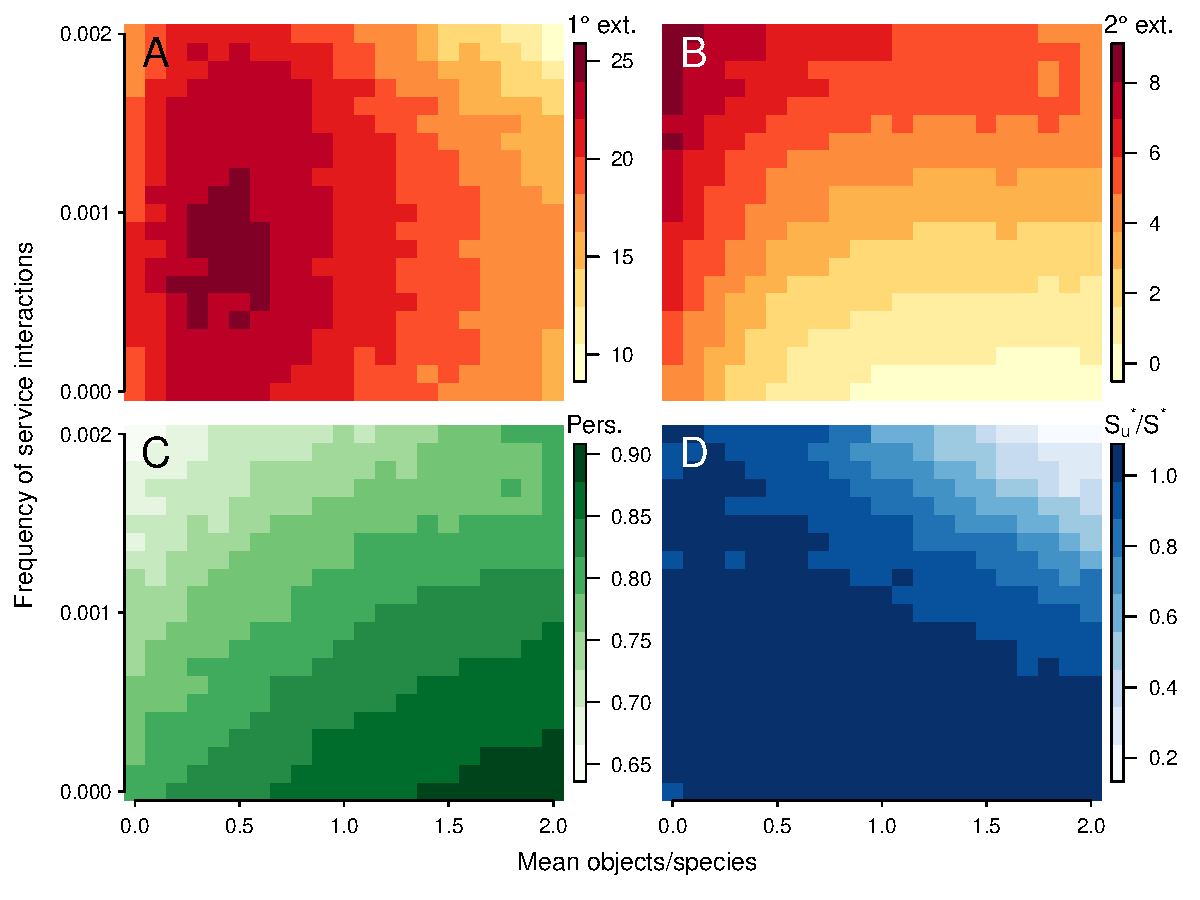
\includegraphics[width=0.5\textwidth]{fig_engineers3.pdf}
\caption{
A. Extinction rate and 
B. species persistence for communities with increasing frequencies of service interactions and average number of objects made per species $\eta$
}
\label{fig:engineers}
\end{figure}

% \noindent \textbf{Beyond engineering}
%NOTE: THIS IS DISCUSSION MATERIAL

%EVOLUTION: CITE LOEUILLE, Fussmann, Allhoff 2013,2015; Brannstrom




While the importance of engineering timescales has been emphasized previously \cite{Hastings2007}, redundancy in the effects of engineers has not \cite{Lawton1994}.
We argue that redundancy may be an important component of highly engineered systems, and particularly relevant when there exists a positive feedback between the effects of engineers on their fitness \cite{Cuddington2004}.
For example, over evolutionary time adaptive radiation of successful engineering clades may lead to increased redundancy, and this may feed back to positively influence the radiation.
The vast majority of contemporary ecosystem engineering case studies focus on single taxa, such that redundant engineers appear rare \cite{Lawton1994}.
However if we consider longer timescales, it is this type of dynamic that likely facilitated the global changes induced by cyanobacteria in the Proterozoic \cite{Schirrmeister2013} among other large-scale engineering events in the history of life.
Engineering redundancies are likely important on shorter timescales as well.
For example, diverse sessile epifauna on shelled gravels in shallow marine environments are facilitated by the engineering efforts of their ancestors, such that the engineered effects of the clade determine the future fitness of descendants \cite{Kidwell1986}.
In the microbiome, redundant engineering may be very common due to the influence of horizontal gene transfer in structuring metabolite production \cite{Polz2013}.
In these systems, redundancy in producing shared metabolitic resources may play a key role in community structure and dynamics \cite{Kallus2017,Muscarella2017}.



%Closing
Together, the results of our model point to the importance of considering diverse interactions both between species and as mediated through changes to the environment via engineering.
We suggest that including the effects of engineers, either explicitly as we have done here, or otherwise, is vital for understanding the inter-dependencies that define ecological systems.
As past ecosystems have fundamentally altered the landscape on which contemporary communities interact, future ecosystems will be defined by the influence of ecosystem engineers today.
Understanding their role is thus tantamount to understanding our own.\\


% \begin{matmethods}

\section*{Materials and Methods}
  \footnotesize{
  % \noindent \textbf{The ENIgMa Model}\\
  We model an ecological system with a network where nodes represent \emph{ecological entities} such as populations of species and or the presence of inanimate objects affecting species such as (examples).
   % and links represent interactions between them.
  Following Pilai et al. \cite{Pillai2011}, we do not track the abundances of entities but only track their presence or absence.
  The links of the network represent interactions between pairs of entities (x,y).
  We distinguish three types of such interactions: x eats y, x needs y to be present, x makes object y.


  The model is initialized by creating $S$ species and $O = \eta S$ objects, such that $N=S+O$ is the total number of entities and $\eta$ is the number of objects per species in the system.
  For each pair of species (x,y) there is a probability $p_e$ that x eats y and probability $p_n$ that x needs y.
  For each pair of species x and object o, there is a probability $q_e$ that x eats o and a probability $q_n$ that species x needs object o..
  Additionally, each species makes a number of objects that is drawn from a Poisson distribution with mean $\mu = \eta e(e-1)^{-1}$ where $e$ is Euler's number.
  Once the number of objects per species is determined, each object is assigned to a species independently.
  This means that there multiple species may make the same object, and that may be some objects that are not made by any species.

  In addition to interactions with ecosystem entities, there can be interactions with a basal resource, which is always present.
  The first species always eats this resource, such that there is always a primary producer in the pool.
  Other species eat the basal resource with probability $p_e$.
  Species with zero assigned trophic interactions are assumed to be primary producers.

  We then consider the assembly of a community which at any time will contain a subset of entities in the pool and always the basal resource.
  In time, the entities in the community are updated following a set of rules.
  A species from the pool can colonize the community if the following conditions are met:
  1) all entities that a species needs are present in the community, and
  2) at least one entity that a species eats is present in the community.
  If a colonization event is possible, it occurs stochastically in time with rate $r_\rr{c}$.

  An established species is at risk of extinction if it is not the strongest competitor at least one of its resources that it eats.
  We compute the competitive strength of species $i$ as
  \begin{equation}
    \sigma_i = c_\rr{n} n_i - c_\rr{e} e_i - c_\rr{v} v_i,
  \end{equation}
  where $n_i$ is the number of entities that species $i$ needs, $e_i$ is the number of entities from the pool that species $i$ can eat, and $v_i$ is the number of species in the community that eat species $i$.
  This captures the ecological intuition that mutualisms provide a fitness benefit, specialists are stronger competitors than generalists, and many predators entail an energetic cost.
  The coefficients $c_\rr{n},~c_\rr{e},~c_\rr{v}$ describe the relative effects of these contributions to competitive strength.
  In the following, we use the values $c_\rr{n} = \pi,~c_\rr{e}=\sqrt{2},~c_\rr{v}=1$, such that the competitive benefit of adding an additional mutualism is greater than the detriment incurred by adding another prey or predator.
  A species at risk of extinction leaves the community stochastically in time at rate $r_e$.

  An object is present in the community whenever at least one species that makes the object is present.
  If a species that makes an object colonizes a community, the object is created immediately, however objects may persist for some time after the last species that makes the object goes extinct.
  Any object that has lost all of its makers disappears stochastically in time at rate $r_o$.

  The model described here can be simulated efficiently with a event-driven simulation utilizing a Gillespie algorithm.
  In these types of simulations, one computes the rates $r_j$ of all possible events $j$ in a given step.
  One then selects the time at which the next event happens by drawing a random number from an exponential distribution with mean $1/\sum_j{r_j}$.
  At this time, an event occurs that is randomly selected from the set of possible events such that the probability of event $a$ is $r_a/\sum_j{r_j}$.
  Then the effect of the event is realized and the list of possible events is updated for the next step.
  This algorithm is known to offer a much better approximation to the true stochastic continuous time process than a simulation in discrete time steps, while providing a much higher numerical efficiency \cite{Gillespie1977}.}
% \end{matmethods}

% 
% 
% \begin{table*}[!t]
% \begin{center}
% \begin{tabular}{ l l l }
% \hline
% Parameter & Definition & Value/Range \\
% \hline
% $\overrightarrow{a}$ & assimilate & \\
% $\overrightarrow{n}$ & need & \\
% $\overrightarrow{i}$ & ignore & \\
% $\overrightarrow{m}$ & make & \\
% \hline
% $e \leftrightarrow i$ & Asymmetric consumption & $p_{ei} = p_i(p_e/(p_e+p_n+p_i)) + p_e(p_i/(p_a+p_i+p_n))$ \\
% $e \leftrightarrow e$ & Symmetric consumption & $p_{ee} = p_e(p_e/(p_i+p_n+p_e))$\\
% $e \leftrightarrow n$ & Trophic mutualism & $p_{en} = p_n(p_e/(p_e+p_n+p_i+p_m)) + p_e(p_n/(p_a+p_i+p_n))$ \\
% $n \leftrightarrow n$ & Non-trophic mutualism & $p_{nn} = p_n(p_n/(p_e+p_n+p_i+p_m))$ \\
% $n \leftrightarrow i$ & Commensalism & $p_{ni} = p_n(p_i/(p_e+p_n+p_i+p_m)) + p_i(p_n/(p_e+p_n+p_i))$\\
% $m \leftrightarrow n$ & Engineering & $p_{mn} = p_n(p_m/(p_e+p_n+p_i+p_m)) + p_m$\\
% $i \leftrightarrow i$ & Null & $p_{ii} = p_i(p_i/(p_e+p_n+p_i))$\\
% \hline
% $\mathcal{N}$ & Number of species + objects & dyn.\\
% $\mathcal{S}$ & Number of species & dyn.\\
% $\mathcal{O}$ & Number of objects & dyn.\\
% \hline
% \end{tabular}
% \end{center}
% \caption{Table of parameters, definitions, and assigned values or ranges.}
% \label{table:param}
% \end{table*}
% 



%
% \textbf{Building the source pool} The source pool interaction matrix $\bm P$ is generated by first setting the number of species in the pool $\mathcal{S}_{\bm P}$ and determining the number of objects $\mathcal{O}_{\bm P}$ that are made by ecosystem engineers.
% The resulting matrix is $\mathcal{N}_{\bm P}\times\mathcal{N}_{\bm P}$ where $\mathcal{N}_{\bm P}=\mathcal{S}_{\bm P}+\mathcal{O}_{\bm P}$, and is subdivided into four quadrants, only two of which play a role here: species-species interactions and species-object interactions (see Fig. \ref{fig:matrix}).
% In these two quadrants, the expected frequency of eat interactions ${\rm E}\{f_\rr{e}\}$ and the expected frequency of need interactions ${\rm E}\{f_\rr{n}\}$ are free parameters, as is the expected number of objects made per species ${\rm E}\{\mathcal{O}_i\}=\eta$.
% Here and throughout, we simplify this parameter space by assuming that the frequency of eat and need interactions for species-species (SS) interactions and species-object (SO) interactions scale as $\phi$, such that ${\rm E_{SS}}\{f_\rr{e}\} = \phi{\rm E_{SO}}\{f_\rr{e}\}$ and ${\rm E_{SS}}\{f_\rr{n}\} = \phi{\rm E_{SO}}\{f_\rr{n}\}$.
% % is given by the parameter ${\rm E}\{\mathcal{O}_i\}=\eta$, which determines how many objects will be present in the source pool.
% % The source pool interaction matrix $\bm P$ is generated by first setting the number of species $\mathcal{S}$ and the expected number of objects that are engineered per species ${\rm E}\{\mathcal{O}_i\}=\eta$.
% For each species, a set number of objects is drawn from ${\rm Poiss}(\eta)$, such that the expected proportion of species that are engineers (species that make objects) is $1-{e}^{-\eta}$.
% If a particular object is randomly and independently drawn for a given engineer from a complete list of all possible objects, such that multiple species -- with some probability -- can make the same object, the expected number of objects is
% \begin{equation}
% {\rm E}\{\mathcal{O}_{\bm P}\} = \mathcal{S}_{\bm P}\eta\left(1 - \frac{1}{{e}}\right),
% \end{equation}
% where $e$ is Euler's number.
% % This allows multiple species to make the same object.
% % If each species makes unique objects, the number of expected objects is $\mathcal{O} = \mathcal{S}\eta$, however because multiple species can make the same object, the realized number of objects will be lower.
% % % To determine whether objects are uniquely made or made by multiple engineers, we assign objects by randomly drawing independently object IDs from $[1:\mathcal{O}_{\rm max}]$ without replacement for each engineer; unassigned objects are discarded.
% % Each engineer is randomly assigned an object, which permits a single object to be made by multiple engineers, such that
% % \begin{equation}
% % {\rm E}\{\mathcal{O}\} = \mathcal{S}\eta\left(1 - \frac{1}{{\rm e}}\right).
% % \end{equation}
% % where $\rm e$ is Euler's number.
% The frequency of $m \leftrightarrow n$ interactions is then calculated as
% \begin{equation}
% {\rm E}\{f_\rr{m}\} = \frac{\eta}{\mathcal{S}_{\bm P}\left(1 + \eta - \frac{\eta}{e}\right)^2}.
% \end{equation}
% Finally the frequency of the ignore interaction is calculated as $\rr{E_{SS}}\{f_\rr{i}\} = 1 - \rr{E_{SS}}\{f_\rr{e}\} + \rr{E_{SS}}\{f_\rr{n}\}$ and  $\rr{E_{SO}}\{f_\rr{i}\} = 1 - \rr{E_{SO}}\{f_\rr{e}\} + \rr{E_{SO}}\{f_\rr{n}\}+ \rr{E_{SO}}\{f_\rr{m}\}$ for species-species and species-object interactions, respectively.
% Pairwise interaction probabilities between both species and objects are then calculated as shown in Table \ref{table:param}.
% These pairwise interactions are assigned randomly from these probabilities between species-species and species-objects independently in both quadrants, such that the source pool matrix has no imbued structure apart from the number of species, the number of objects, and the frequency of each directional interaction type.
% Each source pool is provided a \emph{basal resource} (the first row/column).
% A species with a single trophic interaction to this resource is identified as a pure autotroph (Fig. \ref{fig:matrix}), however the basal resource does not have eat, need, or make interactions itself.
%
%
%
%
% We consider a framework incorporating multiple types of directional interactions between species, which, when paired, represent specific ecological relationships including trophic interactions, service-resource and service-service mutualisms, and commensalisms.
% We also introduce two types of nodes in our depiction of ecological networks: those representing \emph{species} and those representing \emph{objects}.
% Objects must be made by one or more species (here and henceforth refereed to as engineers) and represent a modification to the available niche-space that can be utilized by other species in the community.
% Such alterations are to be considered in the abstract, but in empirical systems could represent an introduced compound, metabolite, or an alteration to the habitat/environment such as, for example, a burrow.
%



%
% %Interaction types
%
% The ENIgMa model consists of four directed interactions:
% $\rr{e}$: eat, which specifies a dependency involving the exchange of biomass,
% $\rr{n}$: need, which specifies a dependency that does not involve biomass flow (e.g. a reproductive service),
% $\rr{i}$: ignore, the null interaction, and
% $\rr{m}$: make, which connects a species to an object that it engineers.
% `Objects' are interactive components that can be made by $\geq 1$ species, and eaten, needed, or ignored by the others.
% The four directed interaction types describe specific dependencies that one species/object has on another, however it is the coupling of two opposing directed interactions that describe familiar ecological relationships (Table 1).
%
% The $\rr{e} \leftrightarrow \rr{i}$ interaction describes a typical predator-prey relationship, where species 1 eats species 2, whereas aside from serving as a resource, species 2 does not interact with (ignores) species 1.
% Of course, a prey's abundance does not \emph{ignore} the effects of predation, however our framework operates at the scale of presence/absence rather than abundance, and we assume that if both species co-occur, they have positive population densities, such that the prey's state (presence/absence) ignores the predator.
% A second type of trophic interaction is described by $\rr{e} \leftrightarrow \rr{e}$, where consumption is symmetric, which could be do to changing roles over an individual's life-history.
% The $\rr{e} \leftrightarrow \rr{n}$ and $\rr{n} \leftrightarrow \rr{n}$ interactions describe service-resource and service-service mutualisms, respectively.
% In the case of the former, one species interacts by way of a trophic interaction, whereas the other is provided a non-trophic need, such is the case in a plant-pollinator relationship.
% Unique to models of ecological networks, the $\rr{m} \leftrightarrow \rr{n}$ interaction describes ecosystem engineering, where a species makes an object, whereas the presence of the object `needs' the presence of the species that makes it.
% Objects can be utilized by other species in the community, providing an indirect dependency that could be facilitated by multiple species (many engineers make the same object) and/or used by multiple species (many species eat or need the same object).
% As we will describe below, engineers can modify the niche space available to the community on timescales that last longer than the species themselves, which is an oft-assumed characteristic of engineering.
%
% We explore the assembly of a novel community that emerges from a species source pool, which is represented by a source pool interaction matrix where all eat, need, ignore, and make interactions are established between all species and objects.
% As such, a set of interactions for a particular species defines how it interacts with any other \emph{a priori}, thereby establishing its potential interaction niche space.
% The source pool is used to seed a novel community, which arises as the result of colonization and extinction rules, the details of which we describe below.
%

\bibliography{aabib}

\end{document}
